\section*{Teleporation in Qiskit}

A 3-Qubit and 3-Cbit register represents the teleportation protocol in Fig. \ref{tc}, with the following specification:

\begin{itemize}
    \item \textbf{Teleport\_Q}: Alice's Qubit to send to Bob
    \item \textbf{Alice\_Q}: Alice's Qubit to be entangled
    \item \textbf{Bob\_Q}: Bob's Qubit to be entangled
    \item \textbf{Alice\_C}: Alice's Classical Bit for measuring Alice\_Q
    \item \textbf{Teleport\_C}: Alice's Classical Bit for measuring Teleport\_Q
    \item \textbf{Teleported\_C}: Bob's Classical Bit for receiving the teleported Teleport\_Q
\end{itemize}
\vspace{1cm} % Adds 1 centimeter of vertical space

The results of the measurement in Fig. \ref{am} and Fig. \ref{bm} bellow.


\begin{figure}[h!]
    \centering
    \caption{Teleportation Circuit}
    \label{tc}
    \begin{minipage}{1\textwidth}
        \centering
        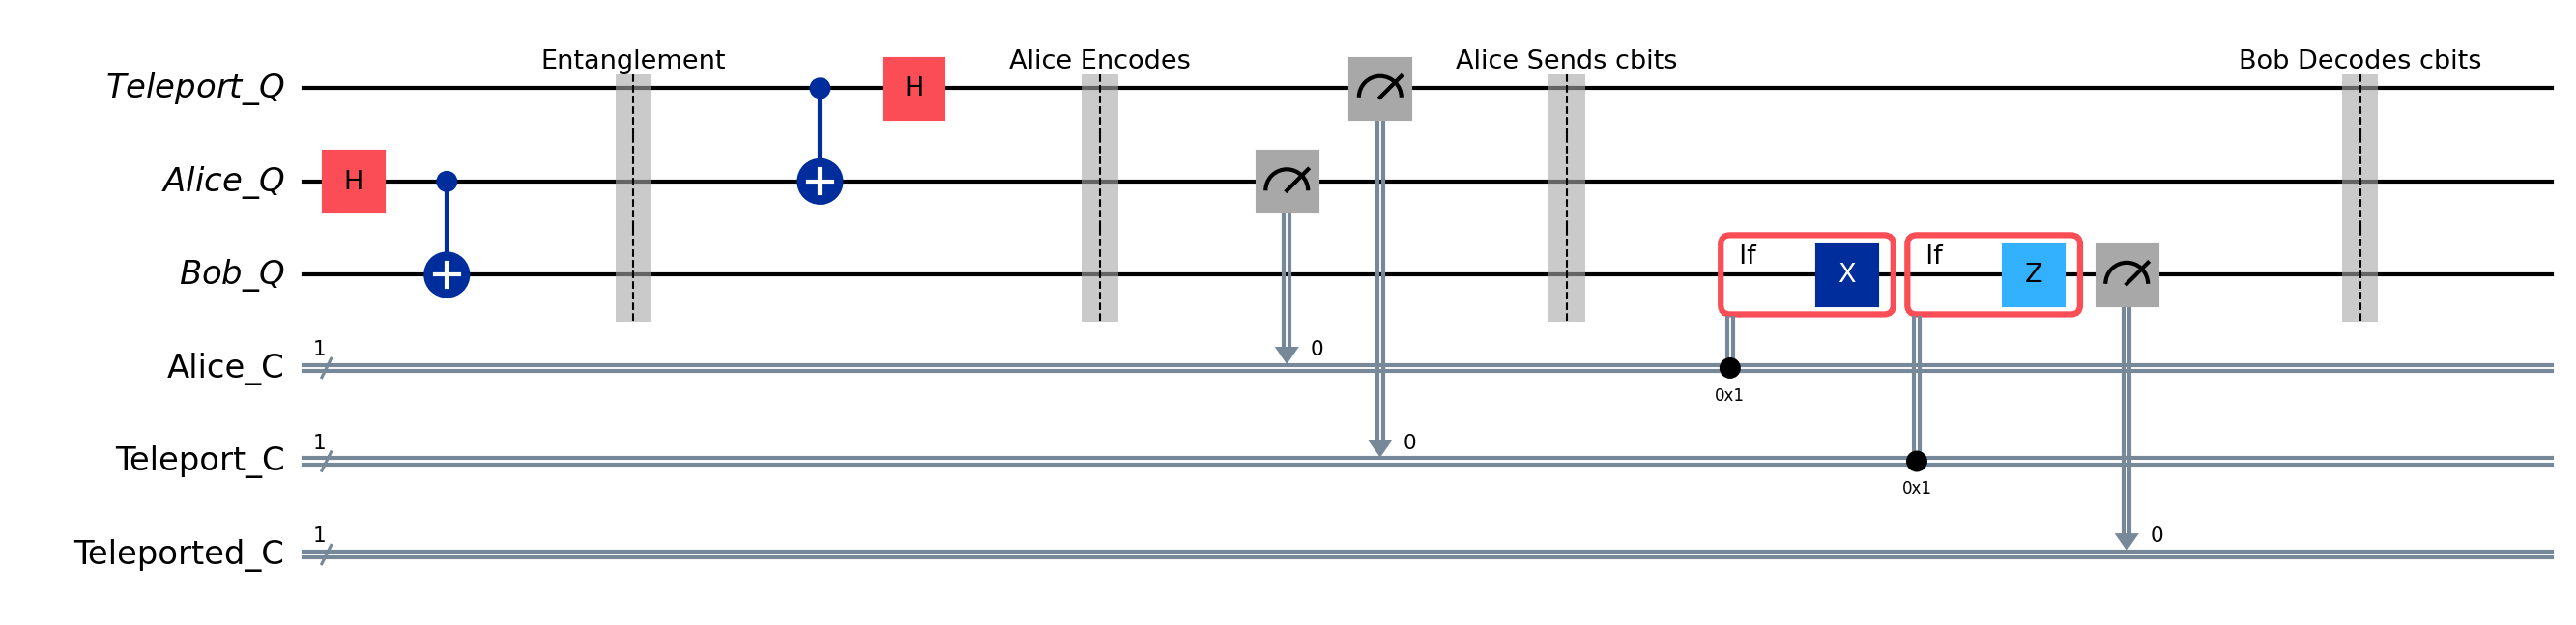
\includegraphics[width=\linewidth]{exercise3/aer_simulator__circuit.png}
    \end{minipage}
\end{figure}

\begin{figure}[h!]
    \centering
    \caption{Alice Measurements}
    \label{am}    
    \begin{minipage}{0.49\textwidth}
        \centering
        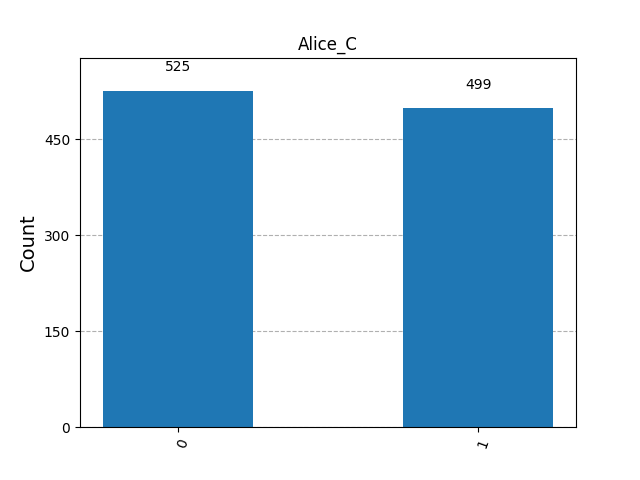
\includegraphics[width=\linewidth]{exercise3/94df8a48-88cc-4ec6-8341-d8ae773c7c37__Alice_C__counts.png}
    \end{minipage}
    \hfill
    \begin{minipage}{0.49\textwidth}
        \centering
        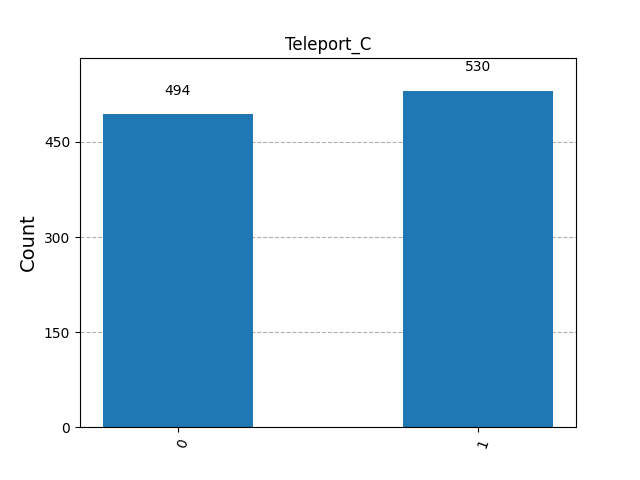
\includegraphics[width=\linewidth]{exercise3/94df8a48-88cc-4ec6-8341-d8ae773c7c37__Teleport_C__counts.png}
    \end{minipage}
\end{figure}

\begin{figure}[h!]
    \centering
    \caption{Bob Measurement of Teleported Qubit}
    \label{bm}    
    \begin{minipage}{0.49\textwidth}
        \centering
        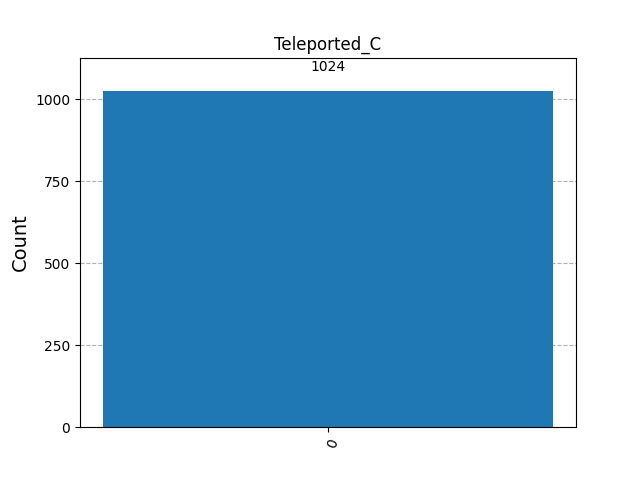
\includegraphics[width=\linewidth]{exercise3/94df8a48-88cc-4ec6-8341-d8ae773c7c37__Teleported_C__counts.png}
    \end{minipage}
\end{figure}

\vspace{6cm} % Adds 1 centimeter of vertical space

We can test the Teleportation Circuit by flipping the initial state of \textbf{Teleport\_Q} qubit, from $|0\rangle$ to $|1\rangle$, and we should expect Bob's measurement to be 1, representing the teleported state of \textbf{Teleport\_Q} to \textbf{Bob\_Q} (Fig. \ref{ctt}). We can validate the Bob's Qubit state which flipped to $|1\rangle$. The results of the measurement in Fig. \ref{am2} and Fig. \ref{bm2} bellow.

\begin{figure}[h!]
    \centering
    \caption{Circuit}
    \label{ctt}
    \begin{minipage}{1\textwidth}
        \centering
        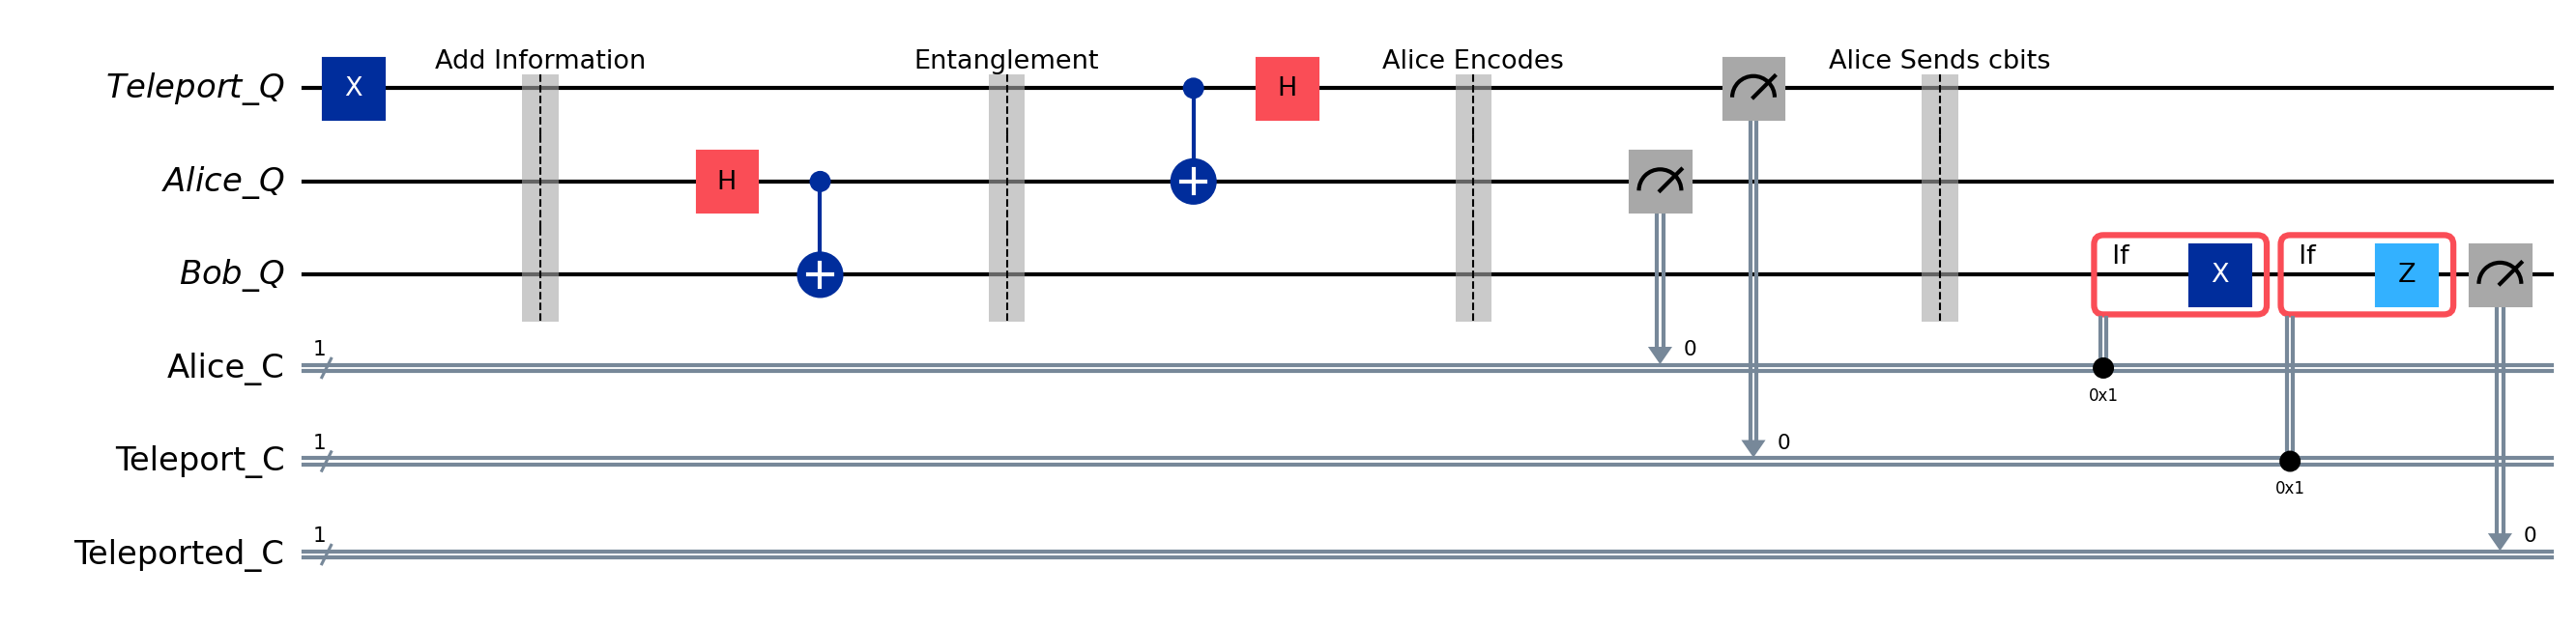
\includegraphics[width=\linewidth]{exercise3/test/aer_simulator__circuit.png}
        \caption*{aer\_simulator(fake\_brisbane)}
    \end{minipage}
\end{figure}



\begin{figure}[h!]
    \centering
    \caption{Alice Measurements}
    \label{am2}    
    \begin{minipage}{0.49\textwidth}
        \centering
        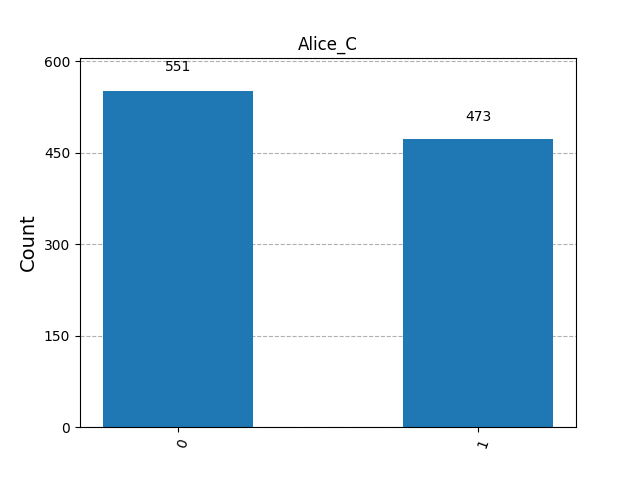
\includegraphics[width=\linewidth]{exercise3/test/51c5350c-8263-4c16-85e8-2cce2067faf0__Alice_C__counts.png}
    \end{minipage}
    \hfill
    \begin{minipage}{0.49\textwidth}
        \centering
        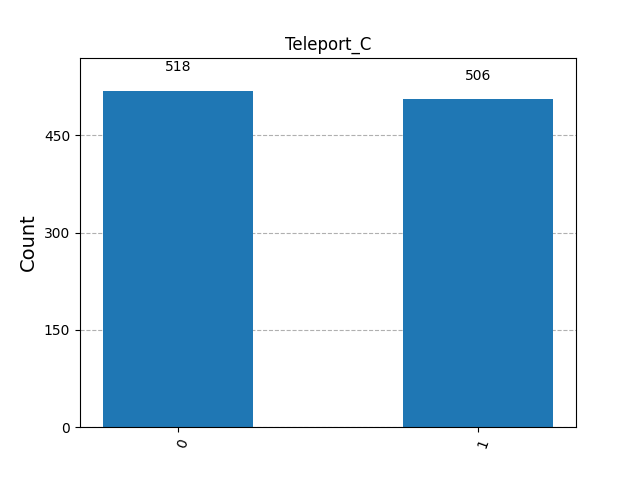
\includegraphics[width=\linewidth]{exercise3/test/51c5350c-8263-4c16-85e8-2cce2067faf0__Teleport_C__counts.png}
    \end{minipage}
\end{figure}

\begin{figure}[h!]
    \centering
    \caption{Bob Measurement of Teleported Qubit}
    \label{bm2}    
    \begin{minipage}{0.49\textwidth}
        \centering
        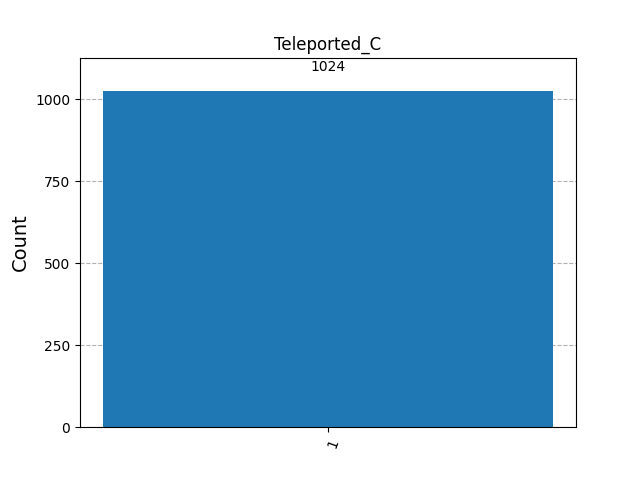
\includegraphics[width=\linewidth]{exercise3/test/51c5350c-8263-4c16-85e8-2cce2067faf0__Teleported_C__counts.png}
    \end{minipage}
\end{figure}

\vspace{5cm} % Adds 1 centimeter of vertical space
